\chapter{Background on Biological Collections}\label{biodiversity_data}


% Biological Collections Data
% ---------------------------
% Characteristics of occurrence data?
%  Punctual data, often obtained in an opportunistic fashion
%  May include collectors field notes.
%  Main assets of a occurrence record: taxon, location, datetime {Graham2004} -> for us, also collectors
%  Biological collections
%  Data collection is typically opportunistic.
% \cite{Hardisty2013}.

% Biological collections
Biological collections (mainly herbaria and natural history museums) are repositories where biological materials, in the form of physical specimens, are systematically deposited and preserved to be used for scientific purposes. 
Throughout this text we use biological collections as a synonym for \textit{Natural History Collections (NHC)}, the later term being more widely adopted in biodiversity informatics literature.
Such collections are typically hosted and curated by institutions like herbaria and natural history museums, which provide appropriate physical infrastructure and human resources for ensuring both the long-term preservation of the collections and their accessibility to the scientific community.
%In addition, these institutions usually count with large networks of associated contributors, including professional collectors and taxonomists.
% Data acquisition: (1) New collecting expeditions; (2) Collections exchanges materials with other institutions

In this chapter we give an overview of how data in biological collections is structured.
We describe the semantics of species occurrence records in section \ref{section:occurrence_data}.
We also discuss some aspects regarding the quality and limitations of such data, and how we deal with these limitations.
Before delving into the characterization of biodiversity data we first review the definitions of some domain-specific terms that will be used throughout this text. 

% =====================
% Terms and Definitions
% ---------------------
\section{Biodiversity-related terms and definitions} \label{section:biodiversity_terms}
\ped{Acham que devo colocar esta seção como apêndice?}

In this work we specifically use definitions from the \textit{International Code of Nomenclature for algae, fungi and plants} (ICN) \cite{McNeill2012}. This document outlines a set of rules and guidelines for scientifically naming and grouping plants, fungi and algae, consisting of a universally adopted reference by the botanical scientific community. Nomenclature best-practices for other groups of organisms are governed by other (though similar) documents.

\paragraph*{Taxonomy.}
Within the domain of biology taxonomy is, in a general sense, the science of classification of organisms. 
Organisms are classified in a hierarchical system, where more specific groupings of organisms are nested within broader ones. 
For an analogy with set theory, a taxonomic classification system can be thought as being similar to a hereditary (or pure) set, in that all members in a set are, recursively, also required to be sets. In our case, however, we allow the existence of non-set objects only in the lowest-level set, which is the most specific grouping of organisms a taxonomist can come up with.

\paragraph*{Taxonomic Rank.}
The taxonomic rank of a grouping of organisms is the level of the taxonomic hierarchy at which it is defined. The most relevant ranks adopted in botany (in descending hierarchical order) are \textit{Kingdom}, \textit{Phylum} (or \textit{Division}), \textit{Class}, \textit{Order}, \textit{Family}, \textit{Genus}, \textit{Species}, as stated in \textit{Art. $3.1$} of ICN.

\paragraph*{Taxonomic Resolution.}
The taxonomic resolution of a biological sample is the taxonomic rank of the most specific taxonomic determination that has been assigned to it.
For instance, if a sample has been determined up to the level of \textit{species}, this rank is also its taxonomic resolution.
As taxa relate to each other on a tree-like hierarchical structure (with each child taxon having exactly one parent, while a parent taxon can have one or more children), taxonomic identities of a specimen at ranks higher than its resolution can be directly determined.
Although this term is not included in the ICN document, we use this definition throughout this text.

\paragraph*{Taxon.}
A taxon is a taxonomic group of organisms at the level of any rank (ICN \textit{Art.1.1}), which are considered by professional taxonomists to form a \textit{taxonomic unit}. Plural is \textbf{taxa}.

\paragraph*{Species.}
Species is one of the taxonomic ranks organisms can be determined by professional taxonomists as belonging to. It is regarded to be a basic unit of taxonomic classification, although organisms can be further classified in lower-hierarchy taxonomic ranks (infraspecific ranks).
Differently from other ranks, the name of a species is composed using a binomial nomenclature system, in which the name of the genus it belongs to is appended to a \textit{specific epithet}.
Examples of species names are \textit{Caryocar brasiliense}, \textit{Myrcia guianensis}, \textit{Solanum lycocarpum}.

\paragraph*{Specimen.}
When botanists sample organisms in the field they either collect part of the organism (\textit{e.g.} a branch of a tree), the entire organism (\textit{e.g.} the entire body of a weed) or multiple individuals of the same type (\textit{e.g.} a bunch of identical, very small-sized mosses). 
Any of these collected biological materials is an evidence of the existence of a particular organism at some place and time, and should be properly deposited in a biological collection. A specimen is defined as one of such evidences, and refers to a punctual observation of a single kind of organism. For the formal definition refer to \textit{Art. $8.2$} of ICN. 
Although a specimen could be classified by a taxonomist as being a representative of a given species, this is not a requirement for it to be included in scientific collections. Although taxonomists classify specimens in a best effort manner (the most taxonomically precise as possible), sometimes only higher ranks can be determined. The highest taxonomic rank at which the specimen could be identified is known as its \textbf{taxonomic resolution}.
After properly deposited in a biological collection, each record receives a taxonomic identification that assigns the individual to a taxonomic group (a taxon), in a best-effort manner.







% ===============
% Occurrence Data
% ---------------
\section{Species occurrence data} \label{section:occurrence_data}
Physical specimens stored in biological collections (also referred to as \textit{vouchers}) are often associated to complementary information, either annotated by the responsible collectors during the collecting act; or annotated at later stages, after the specimen is deposited in the collection \cite{Chapman2005}.
Information from the collection event include the \textit{date, time} and the \textit{geographic location} where the specimen was collected; the names of the \textit{collectors} who were involved in the collection event; and eventual \textit{field notes} describing contextual remarks, such as weather conditions, habitat features, or the sampling method used.
Other types of information, such as the \textit{taxonomic identity} of the specimen, are determined by taxonomists after the biological material is incorporated to the collection.
The taxonomic identity of a specimen includes not only the taxon name assigned to the sample, but also its nomenclatural status and authorship, the name of the taxonomist who has identified the specimen, and other quality-related information.
As the taxonomic identity of a specimen can be re-evaluated by specialists several times after the first determination (though it requires that the investigator has access to the physical specimen), a history of determinations is usually stored in the collection.
% Occurrence data
Vouchered specimens, together with their associated data, is what scientifically testifies a punctual observation of a species at some location and at some point in time, and is thus referred to as a \textit{species occurrence} record (Figure \ref{fig:occurrences_er}).

\begin{figure}[h!]
  	\centering
    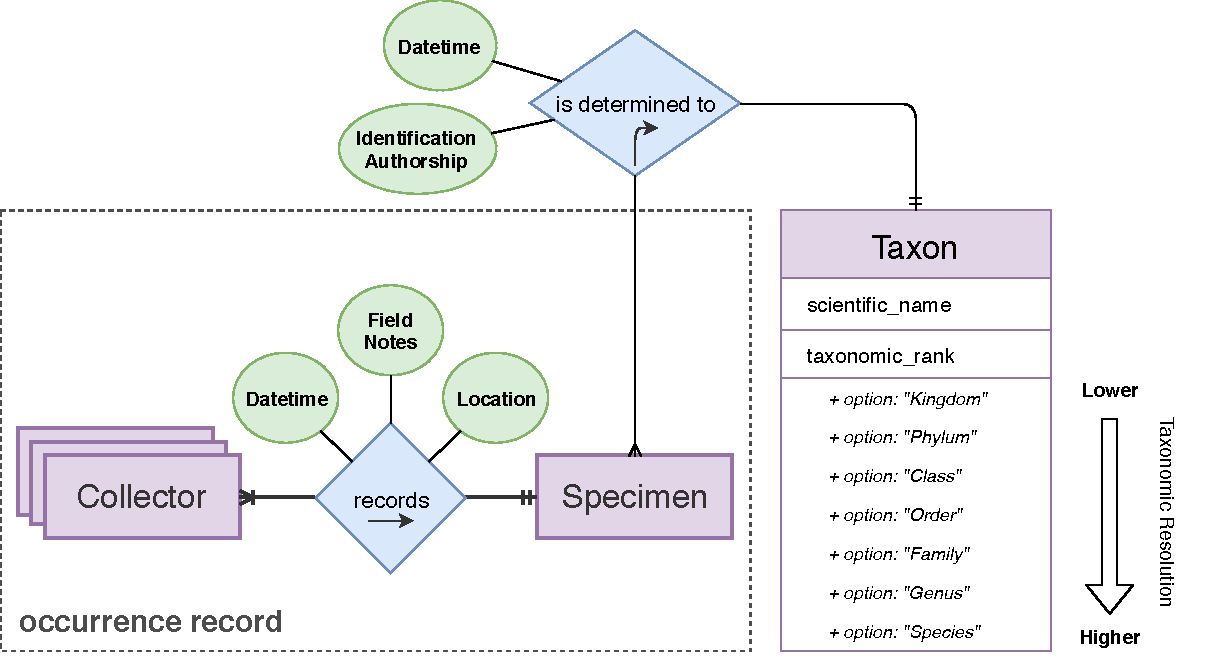
\includegraphics[width=\linewidth]{figures/collections_data/occurrences_er.pdf}
    \caption[Entity-relationship diagram illustrating the main features of occurrence records]{Entity-relationship diagram illustrating the main features of occurrence records. The cardinality of relationships is represented using the Crow's foot notation.}
    \label{fig:occurrences_er}
\end{figure}


With the development of electronic databases over the last $40$ years, many institutions have adopted computerized systems for improving the management and accessibility of specimens-related data \cite{Sunderland2013}.
However, in many regions (including Brazil and China) we face challenges on digitizing information, information is not yet digitized or integrated \cite{Meyer2016}.
% Data sharing intiiatives


%% Citizen science and informal collectors
Although biological collections have traditionally been the most traditional sources of species occurrence data, recent advances in mobile computing technology, associated to connectivity of devices to the wide web, have leveraged the participation of informal groups of nature observers in recording biodiversity \cite{Silvertown2009}.
The nature of such records is similar to those from biological collections in that they are punctual observations of specimens in nature, but also have some important differences: (i) as nature observers usually do not collect biological materials, there are no vouchered specimens, which difficults the taxonmoic determination of the recorded specimen; (ii) taxonomic determinations result from a collaborative community, not and not by professional taxonomists. 






 

Data aggregators publish occurrence datasets, making them more accessible.

% Data issues
Users of occurrence data must be aware of some inherent caveats.
Not all questions can be readily answered with such data, and users must be aware of the impact of those limitations before using it .


 % cite{}
This leads to a set of limitations.
We next review some of those limitations.

\section{Limitations of occurrence data}
% Presence vc presence-absence data
% Collectors Behavior (TerSteege2011)
% Newbold2010
Species occurrence data from biological collections are limited in two important aspects.
First, biological collections contain very limited information on the geographic distribution of organisms, especially for the most imperiled ones, a scenario which is referred to as the \textit{Wallacean Shortfall} \cite{Lomolino2004}.
Many applications of occurrence data require an intensive amount of data to be available.
%
Besides the limitation on the availability of data, another limitation concerns its \textit{quality}.



Distinct aspects of data quality can be affected in multiple stages of its life cycle \cite{Chapman2005}, including the moment of the recording event, its preparation before it can be deposited, the taxonomic determination, data digitization, data storage and analysis.

\subsection{Errors}
Errors in biological collections datasets can be of distinct types, and are more common on the taxonomic identity and spatial information, and can be manually inspected by comparing with collector field notes \cite{Graham2004}.
Determination issues: many specimens are incorrectly identified;
%
\paragraph*{Taxonomic errors.}
The accuracy of taxonomic determinations depend on the expertise of the taxonomists who evaluate the specimens.
Many 
Determination issue, as many specimens are incorrectly identified;
The accuracy of the taxonomic determination depends on the expertise of the taxonomist.
if the identification of the specimen is incorrect, and can be reevaluated if the physical specimen is available.
Typographic (misspelling) errors are particularly common.
They can be dealt with by including authority files containing accepted names 

\textit{geographic errors}, commonly associated to wrong coordinates, imprecise coordinates, unknown datum, null values being interpreted as (0,0) coordinates.
%
\textit{temporal errors}.
%
There are also \textit{typographic} errors, which are common for example in the taxonomic names and in other fields, such as the collector field.



\subsection{Biases}
% collector bias, taxonomic bias, (geographic bias, trait bias, historical bias, seasonal bias) % Daru2017, Haripersaud2009 [Kadmon, R., O. Farber, and A. Danin. 2004. Effect of roadside bias on the accuracy of predictive maps produced by bioclimatic models] [Schulman2007 (collecting bias)->  A mechanism for spatially characterizing collecting bias using Thiessen polygons]
Biological collections are composed of records which have been obtained by distinct people in distinct contexts, having been usually obtained in opportunistic fashion, as opposed to having random sampling designs
Occurrence records are often recorded without random sampling, leading to biases in data.
Biases are introduced in the dataset as an effect of elements that make sampling non-random, such as the detectability, the facility to access areas...
We briefly introduce 4 types of bias (although there are other types as well).
In the context of this work, collector and taxonomic biases are the most relevant.

\paragraph*{Collector bias.}
Not all collectors contribute to the same extent to biological collections.
In fact, a scenario in which a considerable percentage of records are gathered by only a small subset of very productive collectors has been observed in some collections \cite{Daru2017,Carine2012}.
It is a phenomenon in which a small subset of collectors is responsible for the majority of records in a collection.
This unbalance in the representativity of collectors in a collection is what defines the \textit{collector bias}.
%
As collectors have their own particular interests, they tend to prioritize the collection of some taxa, while completely ignoring taxa that are not of their interest.
This is what taxonomic bias is.

\paragraph*{Taxonomic bias.}
Taxonomic bias is intrinsicaly related to collector bias, tending to reflect the interest of the most productive collectors.
The collection is biased towards taxonomic groups most sampled by the most productive collectors.
%
Collectors have their own taxonomic preferences, and thus their collections are not a random sample of the communities they visit.
Some studies have proposed to assess taxonomic bias of collectors by comparing the representativity of each taxon on their sets of records to the herbarium \cite{Haripersaud2009}. %Such approaches give at most a view of how well a collector represents the composition of the collection.
However, if we consider the herbarium itself is composed of contributions of multiple collectors each with particular interests --- and therefore also biased ---, the herbarium is biased, not representing well the natural communities.
As it is very common that collectors towards sampling the highest number of species as possible in localities they visit, the collection is non-random, and rare species tend to be overcollected and common species, undercollected \cite{TerSteege2011}.
Biases of the most productive collectors would be hard to assess.

\paragraph*{Geographic bias.}

\paragraph*{Temporal bias.}

\subsection{Presence/absence data}

\subsection{Data completeness}
% Funk1999 Jacobs2017 Soberon2007

\subsection{Data atomicity}
Some fields in occurrence data are not atomic, which means that multiple values


\section{Improving data quality}
Although data quality can be improved by either prevention or correction, being the prevention considered more effective, as correcting the data is costly\cite{Chapman2005}, prevention is out of our scope, here we limit our scope to correction.
Here we deal with data validation and cleaning of aspects that are most relevant for the modeling we propose.
GBIF has a set of data validation routines, that base on outlier detection, that look for inconsistencies and flag them, but do not overwrite, so that they can be inspected by data user.

Data cleaning depends on the defining the intended use of data (data fit for use).

In the scope of this work, we primarily deal with the entity-resolution problem.

\subsection{The entity-resolution problem}


\cite{Bhattacharya2007}

% Data Aggregators
Gbif provides a data preprocessing routine % https://www.gbif.org/infrastructure/processing





%% As it is common practice for botanists to record each species once during field work, some important ecological attributes such as the species abundance are not to be directly inferred from such data. {check van Gemerden 2005, from Haripersaud2009}


% Biological collections are composed of aggregates of multiple biodiversity surveys, each recorded with particular methodologies
% Records sampled using distinct methodologies can be combined for optimizing data use \cite{VanGemerden2005}.











% ============
% Data quality
% ------------
% [Soberon2004]

% Data quality among collection records is uneven -> worse for large datasets and for datasets composed by multiple sources
% Procedures are needed for correcting problems

% Quality issues: 
%% Determination issues: many specimens are incorrectly identified;
%% outdated taxonomy;
%% georreferencing errors.

% Data atomicity issues:
% Some fields are not atomic: more than one entity is represented as a single data element. 
% In the recordedBy field, Darwin Core standards state that distinct names should be separated by | (delimiter).
% This varies depending on the standard a collection uses. For example, the BRAHMS system recommends using a ';' as the delimiter.
% BRAHMS docs: https://herbaria.plants.ox.ac.uk/bol/brahms/support/documentation

% Identity issues:
% Entities are not guaranteed to have the same ids through distinct datasets.
% Even in the same datasets there may be variations in their names
% this is specially problematic for fields like the collectors field, which is overlooked for most applications of such data. 
% Some standards provide guidelines for including collectors names: last name + first initials...
% However different standards give distinct guidelines and thus name variants are common.
% How to map all name variants to the same entity? -> This leads to the Entity-resolution problem
Some common issues are: (i) including only the name of the first author of the occurrence, and eventually et.al grouping all other collectors;
(ii) format inconsistences when including multiple collectors. Some datasets do not use unique delimiter characters for separating collectors names, and thus affects the process of names atomization.
(iii) As collectors names are usually included in the form of last name followed by first initials, there are many cases of homonymous, especially for very common surnames (e.g. silva, souza,...).
There are also heteronymous, when distinct names variants are assigned to the same person. It can happen that two people have the same last name and their initials are the same (e.g. André Machado Souza or Ana Maria Souza leads to A.M.Souza).
This can also be the result of typos (e.g. souza becoming souza), or simply omiting parts of the name (e.g. if there are two collectors, A.M.Souza and A.P.Souza, omitting the middle initial makes their names indistinguishable).

% Data fit for use

In order to make data fit for its intended use the analyst must perform data cleaning.

% =============
% Data cleaning
% -------------
%[Chapman2005a]

% Why do we need data cleaning? -> We must make data fit for its indended use

% Goal: improving data quality, removing or treating entries that are 

% Adopting standardized collectors names
% Checking collectors itineraries -> look for the spatial pattern of records by the collector


% ================
% References
% ----------------
%% Museum-based informatics{Graham2004}









% Data Quality

% Preparing data 
% Data Selection
% Data Cleaning


% The Entity Resolution problem


% Homonymous names, heteronymous names
% Typographic errors
First, using different naming conventions or occasionally including typographic errors while entering the data in the database leads to multiple variants of name.
Examples of typographic errors are mis
(such as names with typographic errors) homonymous names (a name
